\documentclass{article}
\usepackage[T1]{fontenc}
\usepackage{lmodern}
\usepackage{graphicx}
\usepackage{amsmath,amssymb}
\usepackage[a4paper,margin=2cm]{geometry}
\usepackage[absolute,overlay]{textpos}
\setlength{\TPHorizModule}{1mm}
\setlength{\TPVertModule}{1mm}
\usepackage[indonesian]{babel}
\usepackage{hyperref}
\setlength{\emergencystretch}{2em}
% unit: Halaman 8

\begin{document}

% === Halaman 8 (python/native) ===

Rinaldi M/II4020 Kriptografi

8

• Algoritma (lebih tepat disebut protokol) 

pertukaran kunci Diffie-Hellman (DH) 

berguna untuk berbagi kunci rahasia yang 

sama antara dua entitas yang 

berkomunikasi. 

• Kunci rahasia selanjutnya digunakan untuk 

mengenkripsi pesan-pesan dengan 

algoritma kriptografi kunci-simetri 

(misalnya DES, AES, dll)

• Keamanan algoritma DH didasarkan pada 

sulit menghitung logaritma diskrit dari 

sebuah bilangan bulat besar.

Algoritma Pertukaran Kunci Diffie-Hellman

% deskripsi: gambar native xref 55
\noindent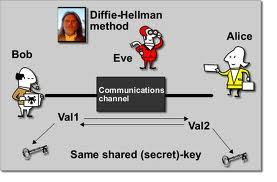
\includegraphics[width=0.85\textwidth]{../../images/python/page_008_img_01.jpeg}

\end{document}
